\chapter{RNA Base Pair Steps}
\label{basepairsteps} 
\bibliographystyle{nar}
Before  the turn  of the  century it  was still  not  conceivable that
knowledge-based potentials  could be obtained for  RNA helical regions
due to the  small amount of crystallographic data  available. This was
not the case  for DNA, where enough data for  such potentials has been
available   since   1998  as   shown   by   Olson  and   collaborators
\cite{olson1998}.   As  pointed  out  in  Chapter  2,  the  number  of
high-resolution X-ray  crystal structures of RNA has  increased by two
orders of magnitude, giving us enough information to develop a dimeric
model of double-helical  RNA with 10 unique base-pair  steps formed by
the canonical G$\cdot$C and  A$\cdot$U Watson-Crick pairs. An extended
model with 21  unique dimeric steps can also  be constructed by adding
the wobble G$\cdot$U base-pair  to canonical G$\cdot$C, and A$\cdot$U,
but for the GU$\cdot$GU (11  cases) and UA$\cdot$UG (20 cases) dimeric
data is still  scarce. An illustration of the  possible unique dimeric
steps which can be formed in RNA as mentioned above is given in Figure
\ref{fig:unique}.

\begin{figure}
\centering
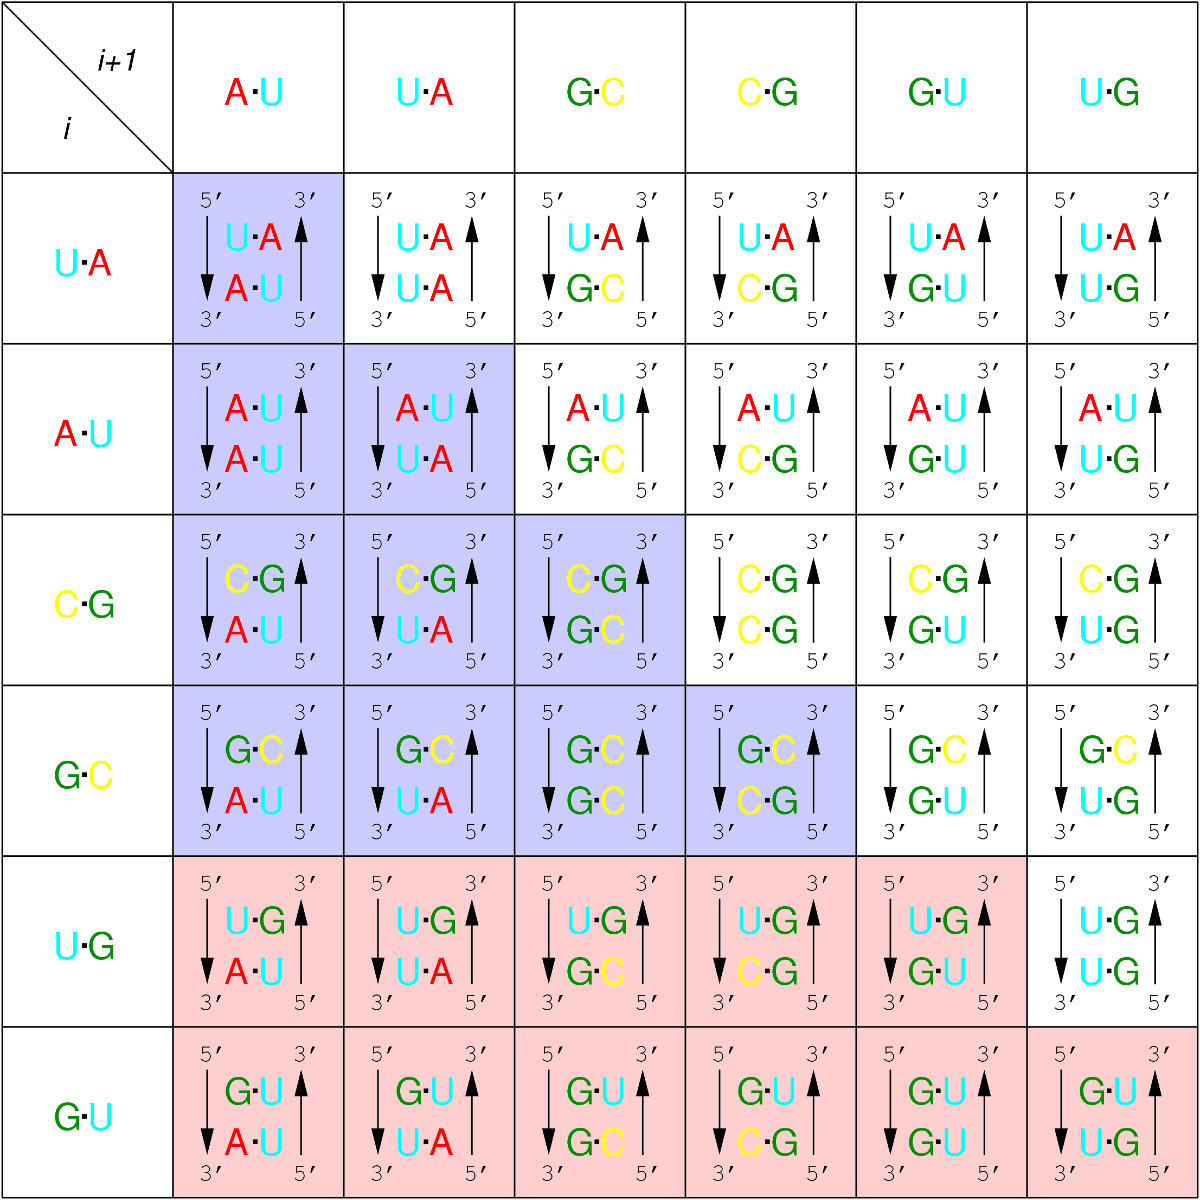
\includegraphics[angle=0, scale=0.4]{Chapter4/unique.png}
\caption{Unique base-pair dimers of RNA formed by canonical G$\cdot$C,
  canonical    A$\cdot$U    Watson-Crick,    and   wobble    G$\cdot$U
  base-pairs.  In purple  boxes the  10 unique  base-pair steps
  formed  by canonical G$\cdot$C  and A$\cdot$U,  and in  beige boxes
  the  additional  11   base-pair  steps  which   result  from
  considering G$\cdot$U  wobble base-pairs as dimer  building block to
  give a total of 21 unique  dimers. The coloring scheme used to color
  the bases is that  used in the NDB, where A is red,  U is cyan, G is
  green, and C is yellow. The first  base-pair in the step in the 5' to
  3' sense is  identified as pair $i$ and the  second is identified by
  $i+1$ as shown in the upper left corner of this figure.}
\label{fig:unique}
\end{figure}  

For the  case of the possible  91 unique base-pair steps  which can be
formed from the seven  dominant base-pairing types discussed in Chapter
3,  we see tendencies of favoured sequences infered from counts of the
available data as will be shown in the next section. 

The results obtained from  the analysis of RNA knowledge-based dimeric
information allow us to explore RNA at the global level, that is, as a
polymer  chain. Therefore we can compute  the  persistence  length  of
some  RNA sequences as shown in the last section of this chapter.

\section{Base-Pair-Steps in Intact Helical Regions}
From  the  dataset  of  base-pairs  described in  Chapter  2  we  also
collected base-pair step information  and focused our attention in the
dimers which are  located in intact helical regions,  those noted as H
in  Figure   \ref{fig:helregxin}.   From  the  data   shown  in  Table
\ref{tab:91steps}  we see that  it's more  common for  a non-canonical
base-pair   to  partner  up   with  a   canonical  base-pair   than  a
non-canonical  one.  The  number of  steps formed  by  a non-canonical
base-pair and a  canonical one is six times higher  than that of steps
formed  by  two non-canonical  pairs.   Some non-canonical  base-pairs
occur exclusively in  the context of a stack  of non-canonicals, e.g.,
GA$_{s}$$\cdot$GA$_{s}$, where two  sheared base-pairs stack together,
or also  on stacks  of a sheared  G$\cdot$A base-pair and  a Hoogsteen
A$\cdot$U  base-pair.  The  majority of  stacks  between non-canonical
base-pairs  occurs  on  dimeric  steps  composed  of  combinations  of
G$\cdot$U  wobble  and  sheared  G$\cdot$A  base-pairs.   Overall  the
majority  of dimeric  steps are  those formed  by  canonical G$\cdot$C
base-pairs  making up  more than  a third  of the  whole.  It  is also
interesting that  more than half  of this kind  of steps is  formed by
GG$\cdot$CC steps.

Overlap values between base-pairs  are given in parentheses along with
the  counts  of dimeric  steps  in  intact  helical regions  in  Table
\ref{tab:91steps}. Looking  at these values the common  trend seen for
overlaps of DNA base-pairs  is mantained, i.e., purine-pyrimidine (RY)
steps have the greatest overlap values, and pyrimidine-purine (YR) the
smallest.   When   the  G$\cdot$U  wobble  base-pair   is  taken  into
consideration the trend remains  true, but the values are considerably
increased, for example for the  GU$\cdot$GU dimer the overlap value is
14.4 \AA$^{\text{2}}$.   The other values  which show a  large overlap
are those of the dimers  composed of sheared G$\cdot$A pairs and those
composed  of sheared G$\cdot$A  and U$\cdot$U  wobble.  The  degree of
overlap doesn't necesarily correlate with greater dimer stabilities as
judged from  the propensities of observed dimers,  for example, wobble
U$\cdot$U pairs prefer to stack with canonical G$\cdot$C pairs showing
a relatively small overlap.

%\begin{sidewaystable}
\begin{table}  
\begin{center}
\scalebox{0.7}{
\begin{tabular}{|c|c|c|c|c|c|c|c|c|c|c|c|c|c|c|}
\hline
C$\cdot$G$_{\text{WC}}$ & G$\cdot$C$_{\text{WC}}$ & U$\cdot$A$_{\text{WC}}$ &
A$\cdot$U$_{\text{WC}}$ & U$\cdot$G$_{\text{w}}$ &
G$\cdot$U$_{\text{w}}$ & A$\cdot$G$_{\text{s}}$ &
G$\cdot$A$_{\text{s}}$ & U$\cdot$A$_{\text{H}}$ &
A$\cdot$U$_{\text{H}}$ & U$\cdot$U$_{\text{w}}$ &
A$\cdot$G$_{\text{WC}}$ & G$\cdot$A$_{\text{WC}}$ & bp$_{i}$/bp$_{i+1}$\\ 
\hline  
604$_{(\text{4.5})}$ & 1335$_{(\text{4.1})}$ & 747$_{(\text{3.0})}$ & 574$_{(\text{2.9})}$ & 77$_{(\text{5.0})}$ & 192$_{(\text{5.3})}$ & 66$_{(\text{6.9})}$ & -- & -- & -- & 18$_{(\text{2.9})}$ & 4$_{(\text{4.8})}$ & 5$_{(\text{4.2})}$ & G$\cdot$C$_{\text{WC}}$\\
 & 608$_{(\text{11.3})}$ & 511$_{(\text{4.1})}$ & 572$_{(\text{9.9})}$ & 161$_{(\text{2.9})}$ & 252$_{(\text{13.5})}$ & 33$_{(\text{10.0})}$ & -- & -- & -- & 69$_{(\text{6.1})}$ & 20$_{(\text{8.8})}$ & 5$_{(\text{7.7})}$ & C$\cdot$G$_{\text{WC}}$\\
 &  & 97$_{(\text{2.0})}$ & 249$_{(\text{3.3})}$ & 20$_{(\text{2.8})}$ & 45$_{(\text{6.1})}$ & 7$_{(\text{7.7})}$ & -- & -- & -- & 2$_{(\text{3.6})}$ & -- & 3$_{(\text{4.3})}$ & A$\cdot$U$_{\text{WC}}$\\
 &  &  & 126$_{(\text{8.4})}$ & 48$_{(\text{2.0})}$ & 79$_{(\text{11.8})}$ & 6$_{(\text{9.5})}$ & -- & -- & -- & 20$_{(\text{8.2})}$ & 1$_{(\text{6.4})}$ & 14$_{(\text{5.3})}$ & U$\cdot$A$_{\text{WC}}$\\
 &  &  &  & 31$_{(\text5.3{})}$ & 42$_{(\text{4.1})}$ & 32$_{(\text{8.3})}$ & 1$_{(\text{5.7})}$ & -- & -- & 5$_{(\text{2.9})}$ & -- & -- & G$\cdot$U$_{\text{w}}$\\
 &  &  &  &  & 11$_{(\text{14.4})}$ & -- & -- & -- & -- & -- & 4$_{(\text{8.8})}$ & 7$_{(\text{9.3})}$ & U$\cdot$G$_{\text{w}}$\\
 &  &  &  &  &  & -- & 13$_{(\text{10.6})}$ & -- & -- & 6$_{(\text{11.1})}$ & -- & -- & G$\cdot$A$_{\text{s}}$\\ 
 &  &  &  &  &  &  & 20$_{(\text{9.1})}$ & 7$_{(\text{3.0})}$ & 2$_{(\text{3.7})}$ & -- & -- & -- & A$\cdot$G$_{\text{s}}$\\
 &  &  &  &  &  &  &  & -- & -- & -- & -- & -- & A$\cdot$U$_{\text{H}}$\\
 &  &  &  &  &  &  &  &  & -- & -- & -- & -- & U$\cdot$A$_{\text{H}}$\\
 &  &  &  &  &  &  &  &  &  & 3$_{(\text{1.7})}$ & -- & -- & U$\cdot$U$_{\text{w}}$\\
 &  &  &  &  &  &  &  &  &  &  & -- & 1$_{(\text{6.3})}$ & G$\cdot$A$_{\text{WC}}$\\
 &  &  &  &  &  &  &  &  &  &  &  & -- & A$\cdot$G$_{\text{WC}}$\\
\hline
\end{tabular}
}
\caption{Unique base-pair steps parameters counts and overlap values
  in RNA helical regions.}
\label{tab:91steps}
\end{center}
\end{table}
%\end{sidewaystable}


%Using information derived from a 3.5 Å parsed subset of the
%BPS (Base Pair Structure) database [2] and so-called “inverse harmonic
%analysis” [3], we have derived elastic force constants for the 21
%unique base-pair steps, and are using this simple scoring potential
%model to simulate the fluctuations of RNA helical structures.

\section{RNA Base-Pair-Steps Database and Webframework}
With the step-parameters from the intact helical regions we can
construct an harmonic energy function model, that is, we can think of
base-pairs  as  rigid  blocks  connected  by a spring  and
described by an harmonic potential function $\Psi(x)$:
\begin{gather}
\Psi (x) = \frac{1}{2}\sum_{i,j} F_{i,j} \Delta x_{i} \Delta x_{j}\\
\Delta x_{i}=x_{i}-x_{i}^{0}
\end{gather}  
Where  the  $x_{i}$  variables  represent  the  displacements  in  the
base-pair steps parameter space,  that is, the displacements in Shift,
Slide, Rise,  Tilt, Roll,  and Twist. It  has been  show by Go  and Go
\cite{go1976} that the force  constants $F_{i,j}$ can be obtained from
the correlation of  displacements in the space of  variables, that is,
they show that these correlations are proportional to $kT$ with a
proportionality coefficient equal to the $i,j$ elements of the inverse
matrix of  second derivatives  with respect to  energy, i.e.,   the $F$
matrix, an analog to the ``classical'' treatment for atoms by Wilson et
al. \cite{wilson1955}.
\begin{gather}
<x_i x_j> = kT (F_{n}^{-1})_{i,j}
\end{gather}
Where $<x_i  x_j>$ stands for  the correlation between  base-pair step
parameter  displacements,  $k$  is  Boltzman's constant,  and  $T$  is
temperature. The total potential for a system of $N$ base-pair steps would
then be given by:
\begin{gather}
U(x_{i}) = \sum_{n=1}^{N} \Psi_{n}
\end{gather}

In order to obtain  quasi-Gaussian distributions of the base-pair step
parameters and also  to exclude protein-induced extreme conformational
deformation  in steps,  we culled  our data  by restricting  it  to be
within a radius  of 3 standard deviations from the  mean value of step
parameters, this data  was used then to obtain  the force constants by
finding the inverse of the correlation matrix.

A  minimal MySQL  database was  created to  store the  mean  values of
base-step parameters,  their standard deviations,  their corresponding
force  constant matrices, and  step deformation  measures such  as the
conformation volume, and RMSD. The purpose of creating the database is
for ease of sharing  information with force-field developers and later
automatization of the process of  data reduction.  The process of data
reduction can be summarized as follows:
\begin{itemize}
\item{Collect a non-redundant dataset of RNA X-ray crystallographic
  structures restricted to resolutions better than 3.5\AA~with up to
  date data from the PDB.}
\item{Find base-pair and base-pair step parameters for all structures
  using 3DNA.}
\item{Find the Leontis-Westhof classification of base-pairs using
  rnaview \cite{yang2003}.}
\item{Build a relational database to relate various classifications,
  for example the Leontis-Westhof classification and the helical
  classification given by 3DNA.}
\item{Select steps present in intact helical regions alone.}
\item{Cull unique base-pair step parameters using a radius of three
  standard deviations.}
\item{Compute means, standard deviations, force constant matrices, and
step deformation measures.}  
\end{itemize}  

The    database   and    its   web-framework    can   be    found   at
\url{http://napoli.rutgers.edu/}. You  will find the table  for the 21
unique dimers  formed by canonical  Watson-Crick G$\cdot$C, A$\cdot$U,
and wobble G$\cdot$U, as shown in Figure ~\ref{fig:average}.

\begin{figure}[htbp]
\centering
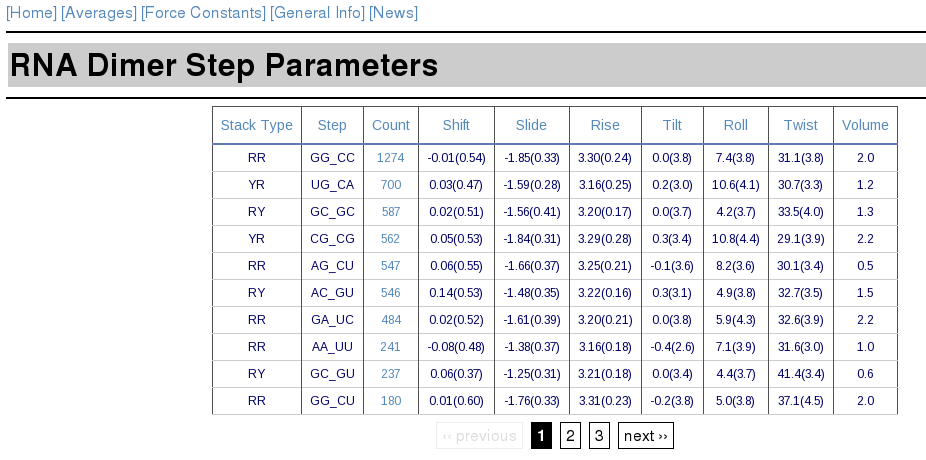
\includegraphics[angle=0, scale=0.4]{Chapter4/average.png}
\caption{Snapshot of the unique base-pair step parameters table for
  intact helical region RNA's, showing the fields that it can be
  sorted by. In this case it has been sorted by dimer step
  counts. There are three stack types purine-purine (RR),
  pyrimidine-purine (YR), and purine-pyrimidine (RY). The steps are
  denoted in a 5' to 3' sense, e.g., GG\_CC stands for a G$\cdot$C
  base-pair stacked on top of another G$\cdot$C pair with intact
  covalent linkage between G's, that is, GpG, and C's, i.e., CpG.}
\label{fig:average}
\end{figure}  

The values in  the table can be sorted by any  of the included fields,
that  is, Stack  Type, Step  Count,  Shift, Slide,  Rise, Tilt,  Roll,
Twist, Volume,  and RMSD. Also  the scatterplot corresponding  to each
step is  displayed when  clicking in the  counts column, along  with a
potential  energy contour  in  the  Roll-Twist plane  at  4.5 $kT$.  A
snapshot  of the  energy contour  for  the GG$\cdot$CC  step from  the
web-framework is shown in Figure ~\ref{fig:contour}.
\begin{figure}[htbp]
\centering
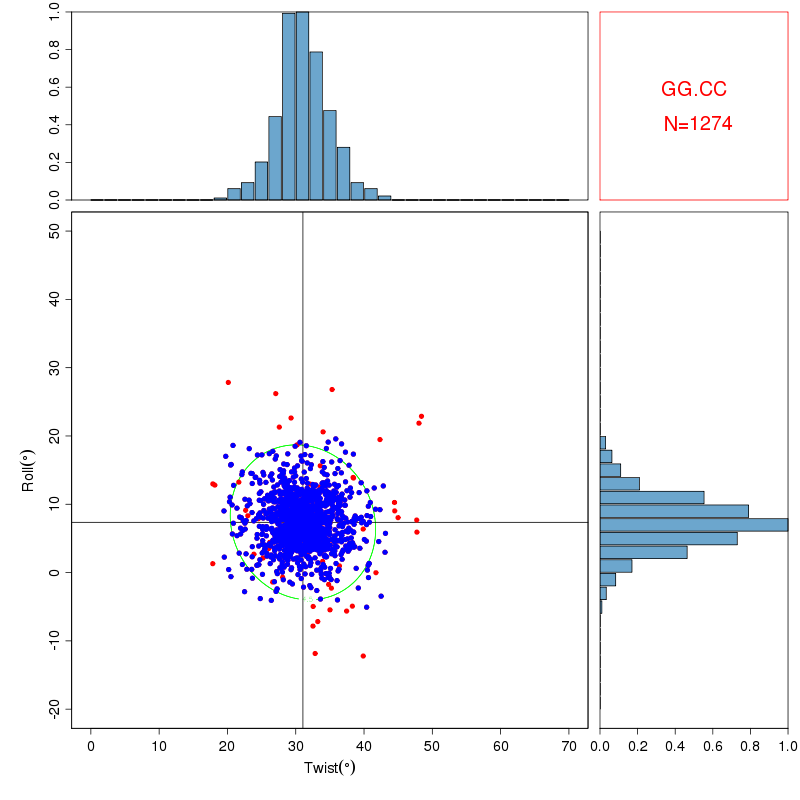
\includegraphics[angle=0, scale=0.4]{Chapter4/contour.png}
\caption{Snapshot from the web-framework of a scatterplot in the
  Roll-Twist plane with an energy contour. The full data before
  culling is show in red dots, and the culled data is shown as blue dots.} 
\label{fig:contour}
\end{figure}

The  other values  included  in  the web-framework  are  those of  the
force-constants corresponding  to the unique steps. A  snapshot of the
force-constant  matrix   for  the  GG$\cdot$CC  is   shown  in  Figure
~\ref{fig:forceconst}

\begin{figure}[htbp]
\centering
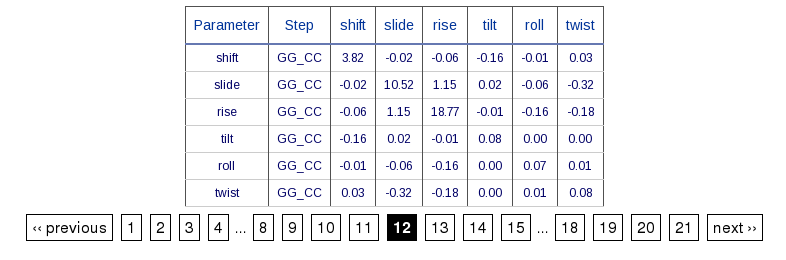
\includegraphics[angle=0, scale=0.6]{Chapter4/forceconst.png}
\caption{Figure showing a snapshot of the RNA Base-Pair Steps
  web-framework where the force constant matrix for the GG$\cdot$CC dimeric
  step is shown.}
\label{fig:forceconst}
\end{figure}  

\section{Persistence Length of RNA}
A quantity commonly used to  quantify the stiffness of polymers is the
so-called persistence  length $a$. To determine this  quantity for DNA
or RNA,  a variety of  theoretical and experimental techniques  can be
used.  Some  common experimental  techniques to determine  $a$ include
electron   microscopy   (EM),   gel   electrophoresis,   sedimentation
velocities, electrical birefringence,  atomic force microscopy (AFM) ,
magnetic  tweezers,  and small  angle  X-Ray  scattering (SAXS).   For
reviews  of  such  techniques  applied  to the  determination  of  RNA
persistence    length,    we   refer    the    reader   to    Hagerman
\cite{hagerman1997}, Abels  et al.  \cite{abels2005},  and Caliskan et
al.   \cite{caliskan2005}.  We  compare  our  simulation results,
based on  the "realistic" model  developed by Olson  and collaborators
\cite{olson1995} to describe DNA, with their findings. The "realistic"
model is dependent  on high-resolution crystallographic data.  Initial
studies started with small numbers  of data for the deformabilities of
the  ten unique  base-pair  steps \cite{olson1995}.   A more  complete
picture applied  to the study of DNA  sequence-dependent deformability
became  available   in  1998  \cite{olson1998}.    The  base-pair-step
deformability  data  for  DNA  has  been constantly  refined  as  more
high-resolution DNA and DNA-protein  structures have been added to the
Nucleic Acid Database (NDB) \cite{balasubramanian2009}.  Although such
data has been available for DNA  since 1998, such was not the case for
RNA, until recently \cite{olson2009}.

The  description of the  ``realistic'' model  along with  a simplified
schema of  the C++ code  developed by Luke  Czapla to implement  it, is
given  in Appendix~\ref{appendix4a}.  Also  in such  Appendix a  brief
account of  various definitions of  persistence length and  the models
generally used to compute it is given.

Using  the mean  values and  force  constants of  RNA base-pair  steps
available at our  web-framework we can use the  ``realistic'' model as
implemented  by  Czapla~\ref{czapla2006}  to compute  the  persistence
length  of chains  of increasing  lengths formed  from the  ten unique
base-pair  steps  of canonical  Watson-Crick  G$\cdot$C and  A$\cdot$U
pairs.   We  used two  rest  states  in  our calculations,  one  which
corresponds to  a naturally straight chain using  the standard dimeric
parameters for  the A-RNA conformation,  that is, $x_{i}^{0} =  \{0, 0,
  3.30,  0,  0,  31.6\}$ with   a  helical  repeat  of  11  base-pairs
\cite{arnott1999}.   The  other  rest  states  used  are  the  average
base-step   parameters   for    unique   steps   obtained   from   our
web-framework. It's  important to  note that one  cannot have  a chain
composed of  pure GC$\cdot$GC  steps, for example,  since the  step in
between two  such steps is  necessarily a CG$\cdot$CG  step, therefore
eight of the  ten chains formed by the unique  base-pair steps will be
mixed, and  only two will be made  purely from a single  kind of step,
that  is, those  chains formed  from the  GG$\cdot$CC  and AA$\cdot$UU
dimers.

As is expected the persistence lengths for naturally straight chains
are larger than the corresponding chains whose rest states are those
coming from the averaged crystallographic data as seen in
Figure~\ref{fig:perVlen}.

\begin{figure}
\centering
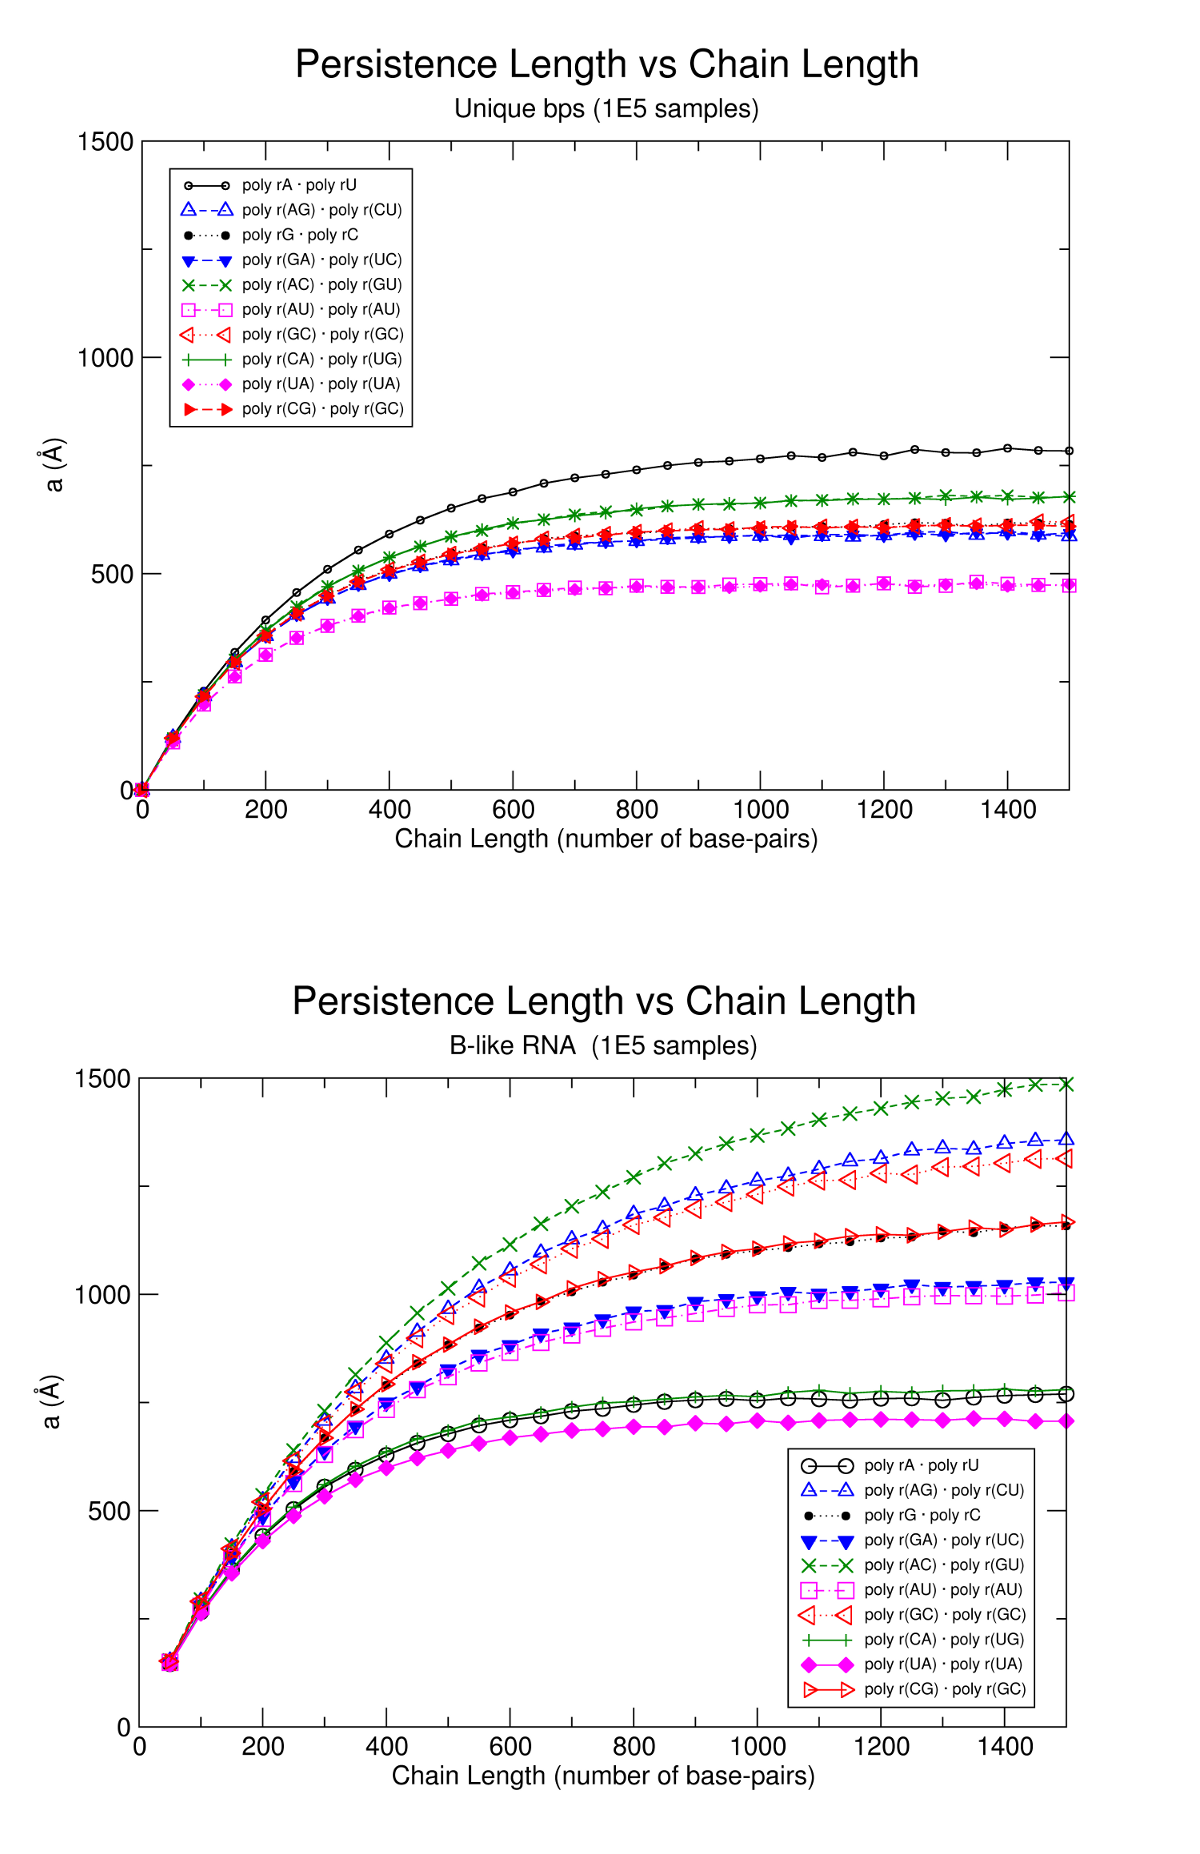
\includegraphics[angle=0, scale=2.8]{Chapter4/perVlen.png}
\caption{In the lower frame persistence length vs chain length in
  base-pairs for naturally straigth chains. In the upper frame the
  persistence length vs. chain length of ``real'' chains.}
\label{fig:perVlen}
\end{figure}


We also computed the persistence length at increasing chain lengths
for a mixed sequence RNA, where we see that a curved.

For comparison to the DNA case we computed the persistence length of a
1000 bp sequence with larger sampling for chains made up from the
unique dimers and using as rest state the values for a naturally
straight chain. We also constructed a random sequence with a
1:1 ratio of A$\cdot$U and G$\cdot$C which is compared to the
values obtained by Abels et al, and those of Hagerman in Table
\ref{tab:compare}. 




%\section{AMBER: Persistence Length of Base-Pair Step Patterns}
%I guess it needs some input here in order to work on latex compilation.



%CHAPTER OUTLINE

%- Methods Paper Results / Trends from counts
%  - Data culled.
%- Step Parameters. Conf Vols, RMSD
%- Equipotential Curves

%- Webserver
%  -table counts
%  -table force constants
%  -potential curves
%  -superimposed structures

%- Persistence Length RNA


% Technical pipeline details
%- Collection of base-pair steps data in helical regions.
%  - Yurong's bps database
%  - Yurong's python 3dnaparser
%  - scripts to change signs, assamble unique steps, and do stats.
%  - scripts to cull data
%  - scripts for deformation score
%  - reconstruction and RMSD calculation
%  - scripts for force-constant-matrices


\bibliography{biblio}

